\documentclass{article}
\usepackage[utf8]{inputenc}
\usepackage{graphicx}

\begin{document}

\begin{figure}[h!]
    \centering
    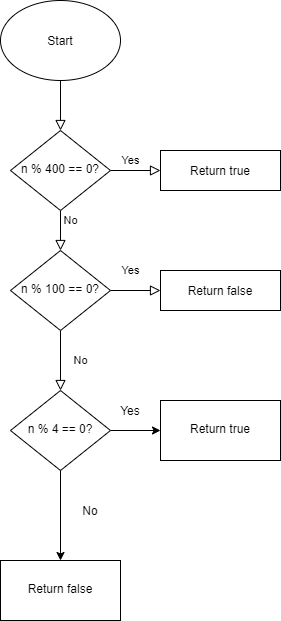
\includegraphics{IsLeapYear_FlowChart.drawio.png}
    \caption[width=0.5]{Flowchart visualizing the IsLeapYear function}
    \label{fig:my_label}
\end{figure}

The algorithm is very simple and starts out by checking if the year modulo 400 is 0 and if so returns true. If not it then checks if the year modulo 100 is 0 and if so returns false. Lastly it checks wherever or not the year modulo 4 is 0 and if so returns true, and if not it then returns false. 

\end{document}
